\section{Experiments}
\label{sec:experiments}
We compare the ExtRA framework with a number of 
baseline methods on extracting  aspect terms from user reviews. 
We first introduce a newly built dataset, the parameter tuning of ExtRA, the baseline methods, and finally the comparisons as well as 
an investigation of the effectiveness of various component of ExtRA.


%\TODO { Comparing with other's aspect extraction results, 
%for example using the human annotated feature words. }
%
%\TODO { Measure the semantic similarity between our extracted top aspect words 
%and the groundtruth aspects. 
%For example, find K nearest neighbors of our extracted aspect words, 
%when K=3, K=5, K=10, how many percent of the groundtruth aspects are matched?
%}
%
%\TODO { End to end aspects summarization, other's results ? }

%\begin{itemize}
%	\item To investigate the effectiveness of different sentence embedding models, we evaluate PV and LSTM with a sentence similarity prediction task. 
%	so that we can decide use which one to
%	 embed sentences to cluster. 
%	 choose PV which is the better one 
%	to encode the review sentences. 
%	We use sentence embeddings of good quality which can capture the semantic similarity between sentences in the  sentence clustering 
%	stage. 
%\end{itemize}
%In this section, we present the results of three experiments. 
%The first one is a comparison of methods for obtaining sentence vectors. 
%In the first step of our framework, i.e., sentence clustering, 
%sentence representation is crucial to the performance 
%and hence critical to overall framework. 
%In particular, we need a vector representation 
%that accurately captures the semantic similarity between sentences, 
%so we test the performance of the methods on a sentence similarity 
%prediction task. 
%The second experiment is the comparison of our framework
%with a number of baselines including the state-of-the-art approaches
%in the end-to-end aspect extraction task.
%The third experiment is a complete aspect-based summarization application using our model.
%
%\subsection{Experiment 1: Comparison of Sentence Embeddings}
%
%%we compares two different sentence embedding models: 
%%long short-term memory (LSTM) and paragraph vector (PV) in this experiment. 
%
%In Stage 1 (\textit{Sentence Representation and Clustering}), we utilize k-means algorithm to cluster review sentences 
%based on the euclidean distance between normalized sentence embeddings, which means the quality of sentence embeddings is  essential to our framework.
%We evaluate two different sentence representation models, which are a long short-term memory (LSTM) based method and \textit{Paragraph Vector} (PV), 
%on a sentence similarity prediction task, namely the English subtask of 
%SemEval-2015 Task 2: Semantic Textual Similarity \cite{agirrea2015semeval}.
%%Since we use the sentence vectors for clustering the sentences based on 
%%their topics, and k-means algorithm uses the distances between the 
%%vectors to determine which cluster each sentence belongs to, 
%%we need the sentence vectors to accurately capture the semantic distance 
%%between the sentences. 
%%For this purpose, we evaluate the models using
%%a sentence similarity prediction task, namely the English subtask of 
%%SemEval-2015 Task 2: Semantic Textual Similarity \cite{agirrea2015semeval}.
%%There are 14,250 data entries, 11,250 for training and 3000 for test,
%%each containing a pair of sentences and a score from 0-5 rating 
%%the semantic similarity of the two sentences.
%%We train our models on all the sentences and 
%%test on the 3000 sentence pairs from the test set.
%The task is to compute the semantic similarity
%for a given sentence pair. 
%%There are totally 14,250 sentence pairs in the dataset, of which 11,250 are for training and 3000 are for test. 
%In the ground truth dataset, each pair is annotated with
%a score from 0 to 5, with 0 indicating that the two sentences are completely dissimilar, and 5 indicating that the two sentences are 
%very similar in semantics. 
%
%To attack this task, we first produce sentence representations
%$h_L$ and $h_R$ for each sentence in the pair using sentence embedding 
%models. 
%Given these sentence representations, we predict the similarity 
%score distribution $\hat{y}$ using a layer of fully connected neural network defined as follows:
%\begin{equation}
%\mathbf{h_s} = \sigma\left(\mathbf W^{(h)}[\mathbf{h_L};\mathbf{h_R}] + \mathbf{b}^{(h)}\right) , \nonumber
%\end{equation}
%\begin{equation}
%\hat{y} = \text{softmax}(\mathbf{W}^{(s)} \mathbf{h_s} + \mathbf{b}^{(s)})
%\end{equation}
%The cost function is defined as follows:
%\begin{equation}
%J(\theta) = \frac{1}{N}\sum_{i=1}^{N}E(y^{i}, \hat{y}^{i})
%\end{equation}
%where $E$ is the categorical cross-entropy loss:
%\begin{equation}
%\label{eq:ce}
%E(y^{i}, \hat{y}^{i}) = -\sum_{r=0}^{R}y_r^{i}log(\hat{y}_r^{i})
%\end{equation}
%In this experiment setting, the dimension of sentence embedding $h_L$ and $h_R$ is set to 300,
%and that of hidden state $h_s$ is 100. 
%The output of \textit{softmax} layer $\hat{y}$ is a probability distribution of 
%ordinal scale of similarity in range $[0,5]$.
%
%%For each sentence pair, both neural network models give us the 
%%independent 300-dimensional sentence vectors; to use this pair of vectors to 
%%predict the semantic similarity, we train an independent predictor backend.
%%The backend is a three-layer feed-forward neural network.
%%It takes the two vectors for the sentence pair given by LSTM or PV as input.
%%The input layer takes the concatenation of the two 300-dimensional vectors;
%%the hidden layer is 100-dimensional; 
%%the output layer is a 6-class softmax, corresponding to the scores of 0 to 5;
%%the loss function is categorical cross-entropy.
%We train LSTM and PV independently with the same number of iterations. 
%We show our results in \tabref{table:semeval} comparing with the winning system of SemEval-2015 task 2, DLS@CU \cite{dlscu}. 
%Note that DLS@CU does not use sentence vectors and cannot be used in our framework.
%%The results are shown in \tabref{table:semeval}.
%\begin{table}
%	
%	\centering
%	\caption{Pearson correlation scores on 5 domains in the standard test set and the mean scores.}
%	\label{table:semeval}
%	\begin{tabular}{|l|c|c|c|c|c|c|}
%		\hline
%		Model & Test 1 & Test 2 & Test 3 & Test 4 & Test 5 & Mean \\ \hline\hline
%		LSTM  & 0.5717 & 0.6329 & 0.6015 & 0.7961 & 0.8147 & 0.6833 \\ \hline
%		PV    & 0.5928 & 0.6681 & 0.6292 & 0.8044 & 0.8419 & 0.7072 \\ \hline
%		DLS@CU & 0.7390 & 0.7725 & 0.7491 & 0.8250 & 0.8644 & 0.8015 \\ \hline
%	\end{tabular}
%\end{table}
%From the results, we can see that 
%PV outperforms LSTM and has fewer parameters.
%%This is probably because the last hidden vector of LSTM is not 
%%a proper representation of the sentence for the semantic similarity task, 
%%due to its emphasis on the last seen word as opposed to earlier words. 
%%We show the effect of different sentence embeddings 
%%in our prominent aspect extraction task in the next experiment. 
%%The performance of different sentence vectors is included in the next experiment.
%\subsection{Prominent Aspect Terms Extraction}

\subsection{Dataset}
We collect our customer review corpora of 6 kinds of product and service
from three popular e-commerce websites, including Amazon, Tripadvisor and Yelp. 
%The data we use in this experiment was gathered from various e-commerce 
%websites, including amazon.com, tripadvisor.com, etc. 
%The reviews are about 6 categories of product or service. 
%The review content is plain English text and we do not use any label
%for training our model. 
%We use human labels for evaluation.  
%are summarized in \tabref{table:dataset}.
The statistics of our corpora are shown in~\tabref{table:dataset}.
\begin{table}[th]
\small
\centering
\caption{Dataset summary.} 
\label{table:dataset}
\begin{tabular}{|c|c|c|}
\hline
Product type & Source & No. of Reviews \\ \hline \hline
hotel        & TripAdvisor & 27,145   \\\hline
mobile phone & Amazon & 3,716  \\\hline
mp3 player   & Amazon & 2,745   \\\hline
laptop       & Amazon & 5,471   \\\hline
cameras & Amazon & 3,077  \\\hline
restaurant   & Yelp & 4,016   \\\hline
\end{tabular}
\end{table}

%We aim to extract $K$ prominent aspects from review texts
%which are most important and representative
%for the given kind of products or services. 
Existing published  datasets\cite{hu2004mining,popescu2007extracting,pavlopoulos2014aspect,ding2008holistic} 
collect fine-grained aspects from reviews,
which are not suitable for evaluating the performance of 
extracted prominent aspect terms. 
Therefore, we build a new evaluation dataset particularly for 
this task.
%
%For most products and services, 3-10 prominant aspects would be 
%enough for the review summarization task, however xx dataset contains dozons of hundreds aspect terms.
%
For each category, we ask 5 annotators who are proficient in English 
to give 5 aspect terms while reading the reviews corresponding to each product type. 
%Our annotated ground truth are all words by design, 
%since the multi-word expressions for aspects  are  very versatile.
%Therefore, we do not show the accuracy of our ExtRA-PV+Phrase model (mentioned in \ref{ourmodels}) in \tabref{table:comparison}.
The manually created ground-truth prominent aspects for each product type are shown
in \tabref{table:labels}.


	\begin{table}[th]
		\small
		\centering
		\caption{Ground-truth. Each row is provided by one annotator.}
		\label{table:labels}
		\begin{tabular}{|c|l|}
			\hline
			\multirow{5}{*}{hotel}
			& room price location service utility \\
			& room service price food location  \\
			& sleep service room price location  \\
			& location price bedroom bath staff  \\
			& room price bath staff location  \\\hline
			
			\multirow{5}{*}{camera}
			& image lens battery memory carry \\
			& picture lens price battery mode \\
			& image price battery design operation \\
			& image lens battery focus storage \\
			& image appearance lens portability battery \\\hline
			
			\multirow{5}{*}{restaurant}
			& location price food service cleanness \\
			& food price location environment service \\
			& price food quietness location staff \\
			& food price service environment location \\
			& food price location service environment \\\hline
			
			\multirow{5}{*}{mobile phone}
			& brand price quality battery screen \\
			& price quality camera touch battery \\
			& quality price design screen carry \\
			& quality price OS battery service \\
			& price quality screen battery color \\\hline
			
			\multirow{5}{*}{mp3 player}
			& price quality sound screen battery \\
			& carry price design sound screen  \\ 
			& price quality carry earphone sound \\
			& quality price battery sound carry \\
			& price quality sound carry screen
			 \\\hline
			
			\multirow{5}{*}{laptop}
			& price quality brand OS battery \\
			& quality price battery memory CPU \\
			& disk memory CPU screen keyboard \\
			& price battery screen CPU performance \\ 
			& quality price appearance battery keyword \\\hline
			\end{tabular}
		\end{table}

\subsection{Parameter Tuning}
\begin{figure*}[t]
	\centering  
	{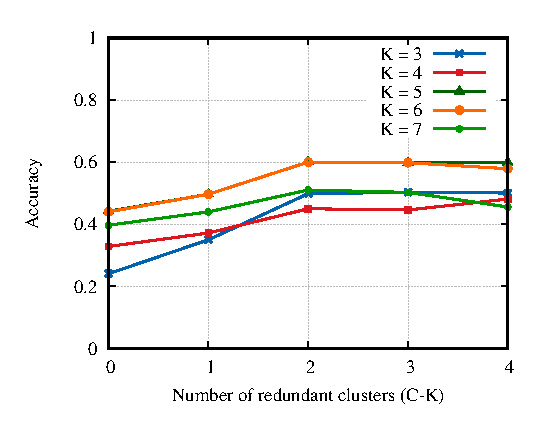
\includegraphics[width=0.8\columnwidth]{data/redundant_clusters_hotel}
\hspace*{1cm} 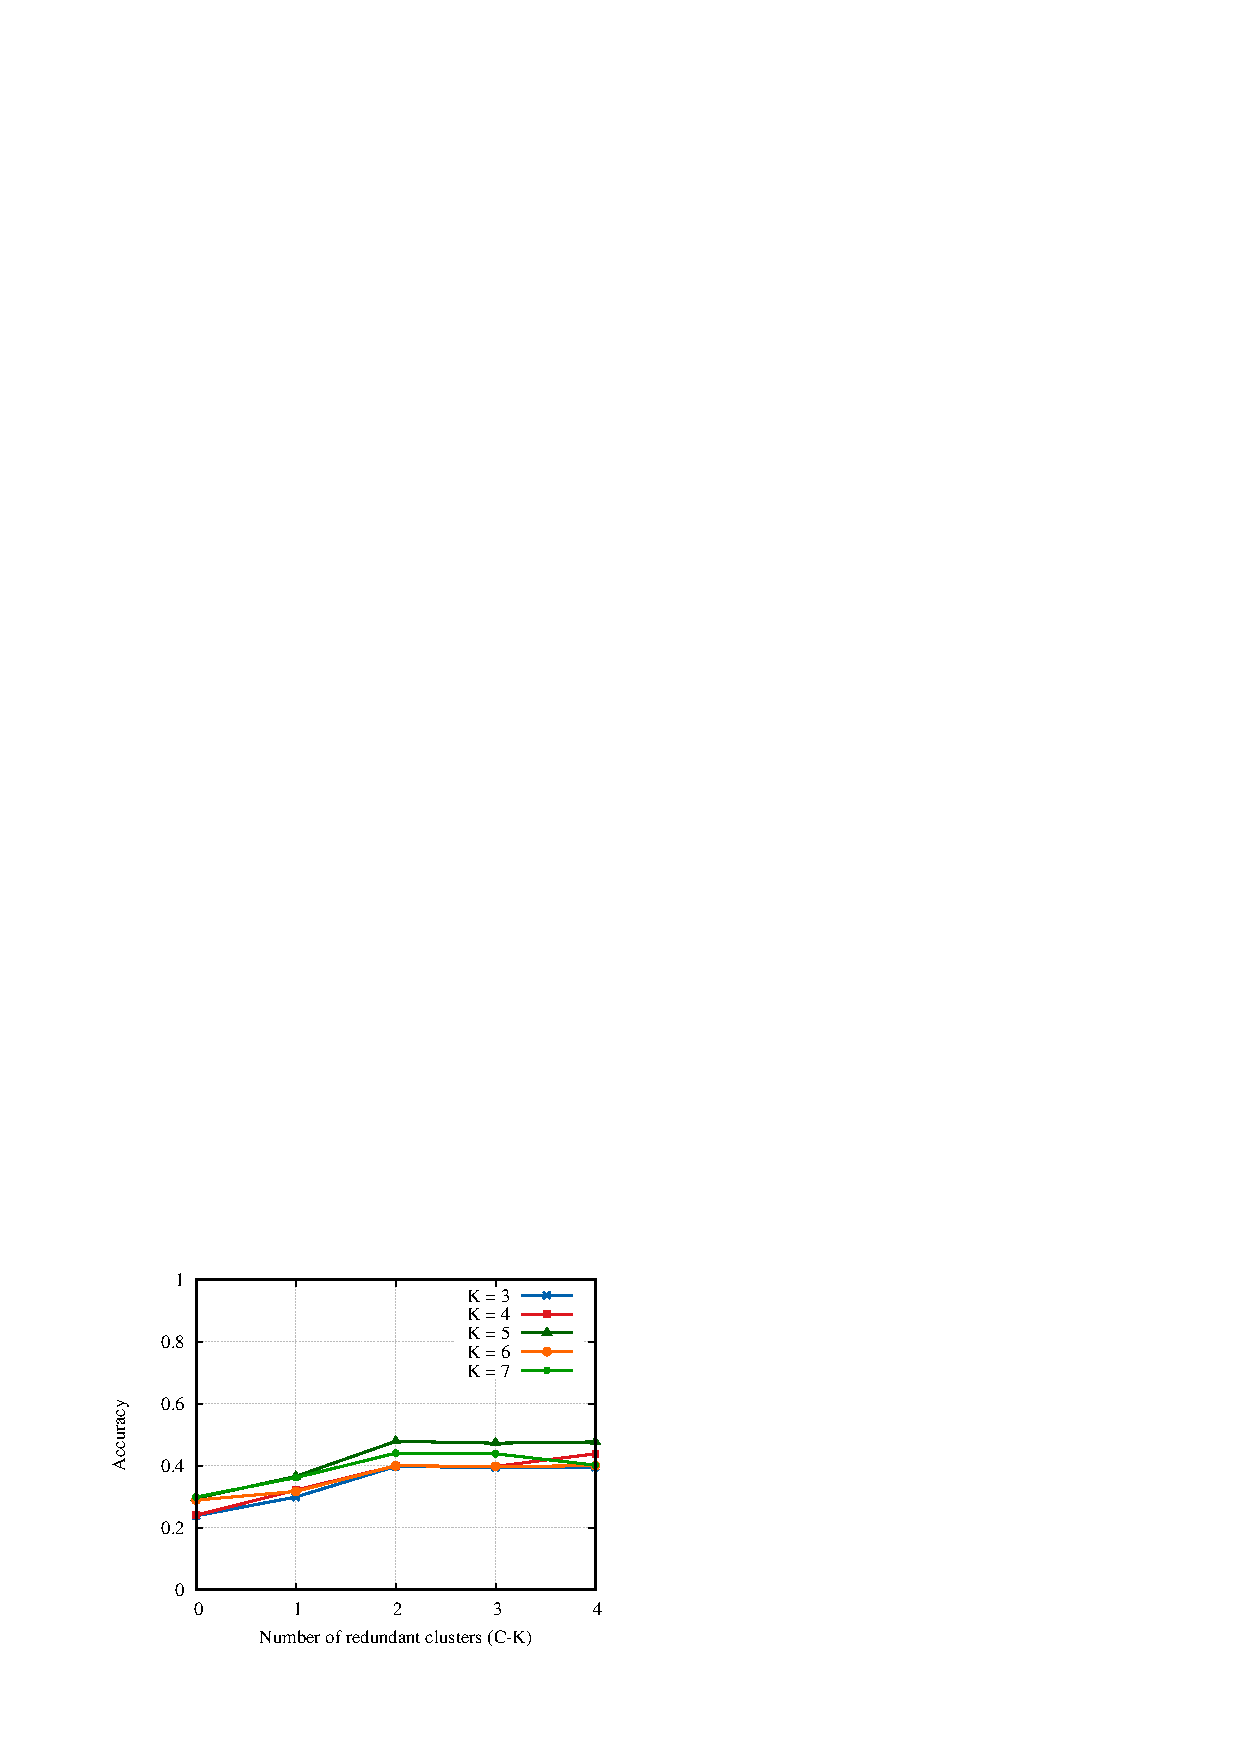
\includegraphics[width=0.8\columnwidth]{data/redundant_clusters_mobile}}
	\vfill
	\caption{The performance of different models when adjusting the 
		number of redundant aspects ($C-K$).  Left: hotel reviews. Right: mobile phone reviews. 	\label{fig:differentc} }

\end{figure*} 
We empirically determine the parameters of our ExtRA $N$, $M$, $C$ in sentence clustering, 
topic modeling and topic clustering stages respectively.
%In this section we conduct experiments to determine the best set of
%parameters of our model, most importantly the constants $N$, $M$, $C$.

\textbf{Number of Sentence Clusters ($N$)}
We expect that sentences in each sentence cluster are about a single review aspect.
%We need to determine the number of sentence clusters $N$.
We use an empirical elbow method to find an optimal $N$ by plotting the loss, which is the sum of euclidean distances from cluster center to each point within the cluster.
\figref{fig:differentn} shows the changes of the loss over different number of sentence clusters.
We conduct the experiments on the \textit{hotel} reviews.
%Note that we do not consider the number of 
%expected prominent aspects here.
%Note that we don't concern about the number of expected aspects 
%in this experiments. 
We find that setting $N$ around 10 is optimal to to achieve the lowest loss, and therefore we set $N$ as 10 in the following experiments.
%to give the lowest loss, the number of sentence clusters should be
%10 or 11.  Therefore, in the following experiments, we set $N$ to be 10.

\begin{figure}[b]
\centering
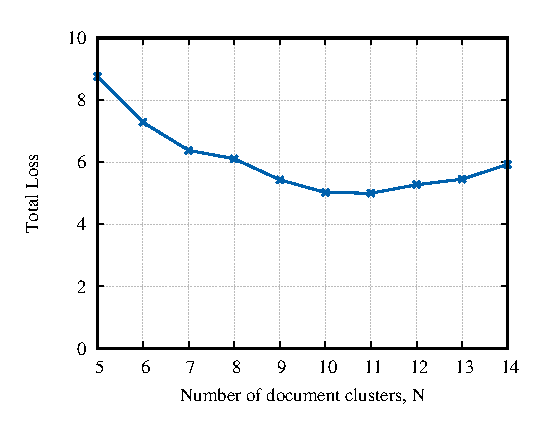
\includegraphics[width=0.8\columnwidth]{data/differentn}
\caption{Selecting $N$, the number of clusters for k-means. The optimal
$N$ is selected to be 10.}
\label{fig:differentn}
\end{figure}

\textbf{Number of Topics within Each Sentence Cluster ($M$)}
In the topic modeling stage, we need to determine 
the number of topics that we would like to model 
for each sentence cluster.
%LDA in our model serves the purpose of isolating the 
%noisy topics and resolving the overlaps between aspects.
As \tabref{table:differentm} shows,
the performance of  our framework is insensitive to $M$.
\begin{table}[t]
	\normalsize
	\centering
	\caption{The effect of different $M$ \FX{Need to update to new results}}
	\label{table:differentm}
	\begin{tabular}{|c|c|c|c|c|c|}
		\hline
		$M$ & 5 & 8 & \textbf{10}& 12  \\\hline
		Accuracy & 17/25 & 16/25 & 17/25 &16/25 \\\hline
	\end{tabular}
\end{table}
%we find that different number of LDA topics
%doesn't have much effect on the end-to-end performance.
%Consider the 25 manually annotated words again,
%the difference between the three numbers is only 
%1 out of 25 words.
Therefore, we set $M$ as 10 in our following experiments.


\textbf{The Number of Topic Clusters ($C$)}
As mentioned in \secref{sec:topic_clustering}, 
we obtain $C$ topic clusters in the topic clustering stage, 
where $C$ is larger than $K$ 
for removing redundant and noisy topic cluster in the following steps.
We demonstrate the effect of different $C$ by adjusting the number of redundant topic clusters ($C-K$) with different selected $K$ in \figref{fig:differentc}.
%In this section we demonstrate the effect of these redundant clusters.
%We show 
%In , we show the accuracy with different 
%redundancy $C-K$, 
$C-K$ is in range $[0,4]$, and $K$ is in range $[3,7]$. 
We can see that it is adequate to set $C-K$
as 2, and our framework would not benefit from removing more topic clusters.
%It can be seen that 2 redundant clusters are sufficient and 
%more redundancies can't improve the performance.

\subsubsection{Baseline Models and Our ExtRA} 
We introduce four baseline models for aspect extraction:
LDA~\cite{Blei2003LatentDA} and BTM~\cite{cheng2014btm} are two simple topic modeling-based methods;
D-PLDA \cite{moghaddam2012design} is a representative for joint aspect-sentiment models;
MG-LDA \cite{titov2008modeling} is a representative for aspect extraction topic models.
We also investigate two variations of our ExtRA model, i.e. ExtRA-LSTM and ExtRA-PV, 
to certify that the using PV is better than using LSTM-based sentence representation.
Note that we use BTM as our topic modeling method in ExtRA.
%We run the above models on the review data for each product type separately. The number of aspects is fixed to 5.
%The number of expect prominent aspects $K$ is fixed to 5.

\paragraph{LDA and BTM}
We use LDA and BTM as two basic topic modeling based methods. 
Considering a given product type or service, 
we treat each review as a document and perform vanilla LDA and BTM on 
the reviews to extract $K$ topics.
Then, we select the words with highest probabilities in each topic as our extracted aspect terms.


%We treat each review as a document and run on the whole corpus (single product type). 
%The number of topics is set to 5 for model comparison.

\paragraph{D-PLDA}
D-PLDA \cite{moghaddam2012design}, 
is a variant of LDA models, which is designed specifically for modeling topics from user reviews.  
D-PLDA only considers opinion-related terms and phrases, 
and nouns and phrases are controlled by two separate hidden parameters. 
%There is a dependency from hidden parameters for adjectives to the one for nouns.
The hidden parameters of adjectives are depended on the parameters of nouns.
We use D-PLDA as a representative for such models joint extracting aspect and sentiment.

\paragraph{MG-LDA}
To compare our model with a popular, well-performed model designed particularly for aspect extraction, 
we use MG-LDA~\cite{titov2008modeling} as a sophisticated baseline method. 
MG-LDA can also models topics at different granularities. 
For fair comparison among different models, the number of target aspects $K$ is set as 5.
The hyper-parameter of MG-LDA (global topics) is set to 30 with fine-tuning.

\paragraph{ExtRA models}
\label{ourmodels}
The dimension of our sentence embeddings is set as 300.
We refer our models which are fed with different sentence embeddings as ExtRA-PV and ExtRA-LSTM, respectively.
Note that both of them utilize BTM as the topic modeling method in Stage 2.
%For sentence vectors (both LSTM and PV), the dimensionality is set to 300.
%We refer such models as ExtRA-PV and ExtRA-LSTM. 
The parameter configurations in our experiment in \tabref{table:comparison} are as follows:
 $K=5$, $N=10$, $M=10$, and $C=7$.
Note that we train the sentence embeddings merely on review texts and do not use extra data. 
%The number of sentence-level clusters is set to 10; the number of LDA topics is 10; the number of final word clusters in the clustering phase is 7 and is later reduced to 5 in the ranking phase. For training the sentence vectors, we do not use any extra data, all the word and sentence vectors are trained on the set of reviews for a single product type. 

\subsubsection{Aspect Term Extraction Comparison}
The labels provided by the annotators are aggregated together without removing duplicated words, so we have 25 words in total.
This is to ensure that the information about the different importances of aspects is preserved.
When evaluating the models, 
we compare the 5 aspect words generated by the models with those provided 
by the annotators. 
We calculate the portion of words among the 25 labels that 
are correctly generated by the model as the \textit{accuracy} of the model.

%\begin{figure*}[t!]
%\centering
%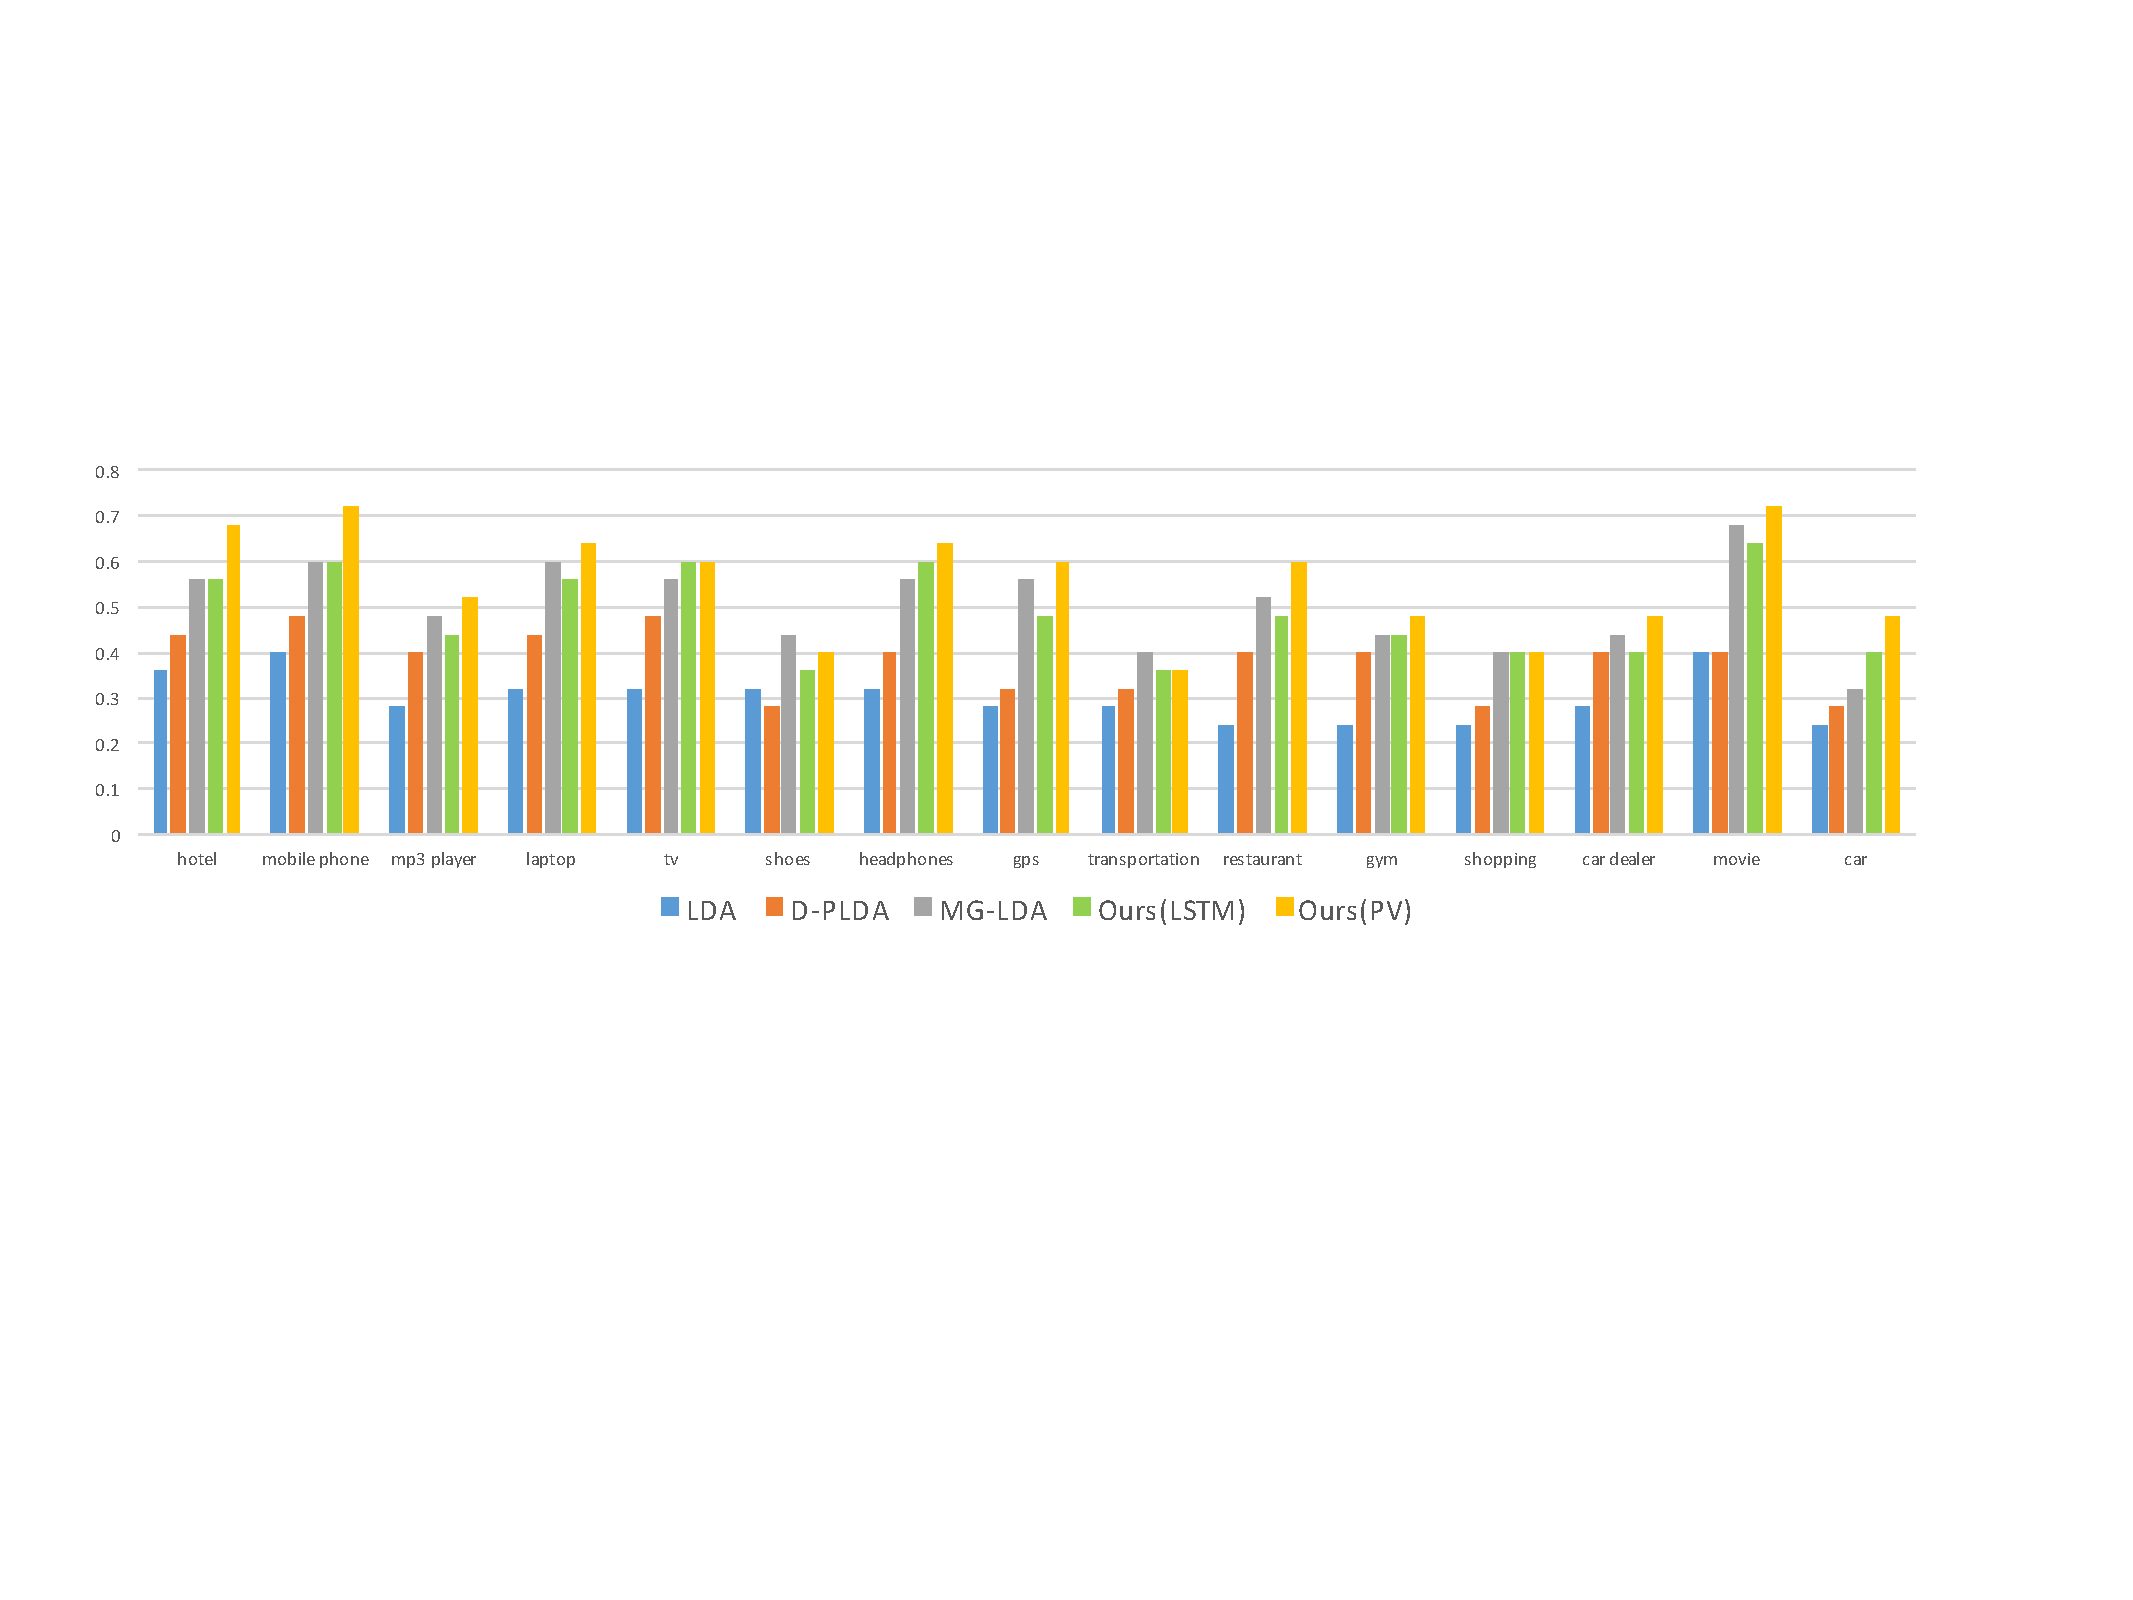
\includegraphics[width=2.0\columnwidth]{figures/results}
%\caption{Comparison of accuracies from different models on aspect extraction.}
%\label{fig:results}
%\end{figure*}  
\begin{table}[t]
	\centering
	\caption{Comparison of \FX{not accuracies} accuracies using different models for aspect extraction.}
	\label{table:comparison}
	\begin{tabular}{|c|C{0.7cm}|C{0.8cm}|C{0.7cm}|C{0.8cm}|C{0.8cm}|C{0.7cm}|}
		\hline
		\diagbox[width=7em]{Models}{Types}& hotel & mobile phone & mp3 player & laptop & camera & restaurant  \\ \hline
		LDA & 0.699 & 0.458 & 0.395 & 0.397 & 0.408 &  0.418 \\ \hline
		BTM & 0.509  & 0.474& 0.542 & 0.417 & 0.510 & 0.595 \\ \hline
		D-PLDA & 0.528 & 0.589 & 0.496 & 0.503 & 0.460 & 0.515 \\ \hline
		MG-LDA & 0.590 & 0.640 & 0.539 & 0.638 & 0.622 & 0.625 \\ \hline
		ExtRA-LSTM & 0.621 & 0.576 & 0.541 & 0.618 & 0.609 &  0.607 \\ \hline
		ExtRA-PV & 0.713 & 0.564 & 0.552 & 0.691 & 0.645 & 0.664 \\ \hline
	\end{tabular}
\end{table}


In this evaluation, we compare the performance of our models 
with the baseline models mentioned above. 
The results are shown in \tabref{table:comparison}. 
\ZY{Our model performs better on all products except for mobilephone.}
Our models outperform others in all categories. 
We can also see that ExtRA-PV indeed outperforms 
ExtRA-LSTM, which is consistent to the previous experiment results.
Also, we find that BTM is better than LDA and our framework performs better than the existing state-of-the-art methods.
Especially, since the accuracy of ExtRA-PV is higher than BTM, we claim that our sentence clustering indeed benefit the topic modeling process. 
%Our model with paragraph vector performs better than with LSTM, 
%which is consistent to our result from the previous experiment.

To qualitatively evaluate different models,
we present that the extracted aspect terms (boldfaced) of each models and their candidates with highest scores in \tabref{table:hotel_aspect_words}. 
%The top words, which are chosen as the representatives of the aspects, are shown in boldface. 
{Our framework can be extended to extract multi-word aspects (aspect phrases) by integrating AspVec, which is called ExtRA-PV+Phrase.}
\figref{fig:topiccloud} is the visualization (using TopicCloud toolkit\footnote{Open sourced toolkit is available at \url{https://github.com/askerlee/topiccloud}} \cite{li2017document}) for aspect clusters generated by ExtRA-PV+Phrase model on hotel review.
The portion of area for clusters depends on their distinctiveness score.
Also, the scores of the words in each cluster determine their font-sizes.
With this visualization, the importance of each cluster and word is clearly presented.


\begin{figure}[t]
	\centering
	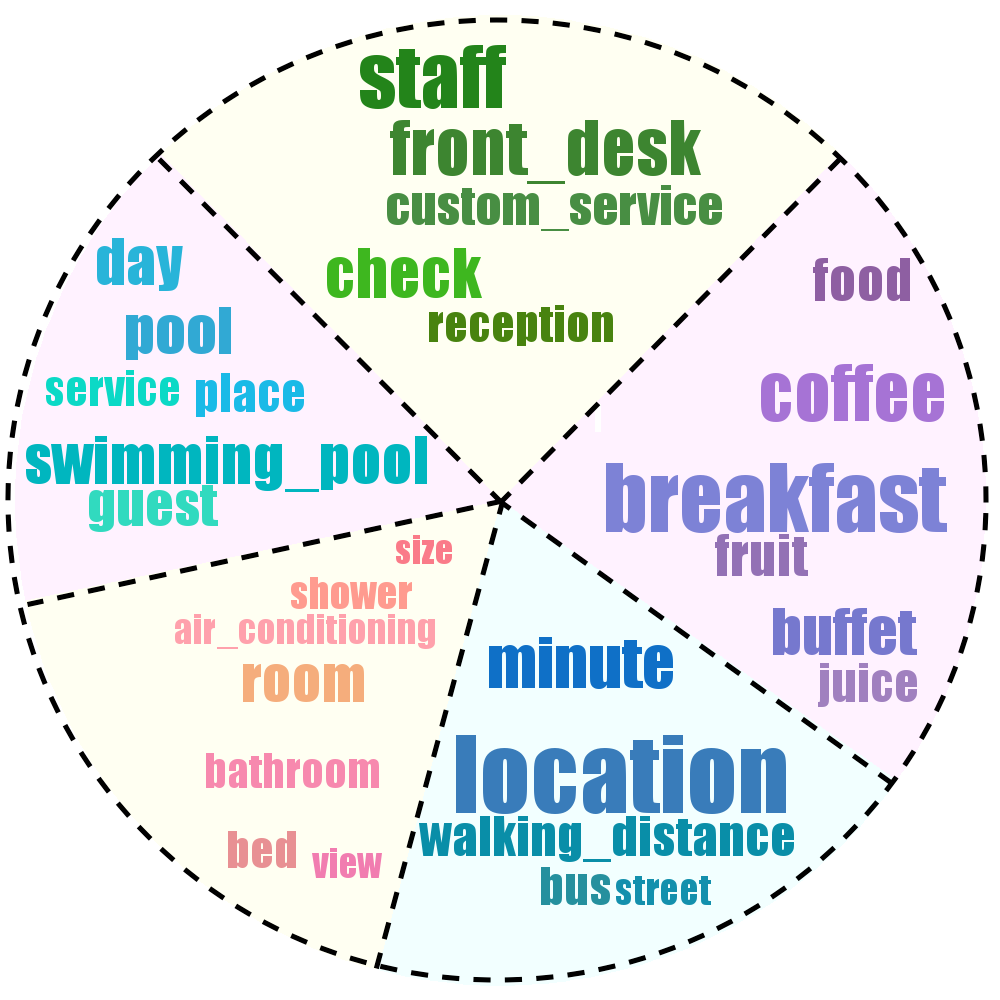
\includegraphics[width=0.8\columnwidth]{figures/topics_hotel}
	\caption{Aspect Cloud: visualization of aspect words and phrases extracted from the hotel reviews.}
	\label{fig:topiccloud}
\end{figure}

\begin{table}[th]
	
\centering
\caption{Top aspect words (with phrases) for hotel reviews by different models}
\label{table:hotel_aspect_words}
\begin{tabular}{|l|l|} \hline
\multirow{5}{30px}{ExtRA-LSTM}
& \textbf{service}, front, desk, reception, concierge, check, gust \\
& \textbf{location}, station, minute, tube, station, bus, distance \\
& \textbf{time}, check, day, desk, charge, book, front, hour, night \\
& \textbf{food}, coffee, buffet, morning, tea, room, fruit, egg, juice \\
& \textbf{bed}, bathroom, size, floor, view, suite, king, book, decor \\ \hline

\multirow{5}{30px}{ExtRA-PV}
& \textbf {staff}, service, room, front, desk, check, concierge \\
& \textbf {food}, breakfast, bar, restaurant, coffee, morning, tea \\
& \textbf {price}, parking, night, place, rate, service, money, star \\
& \textbf {room}, bed, bathroom, size, suite, floor, view, bedroom \\
& \textbf {location}, minute, square, subway, street, block, distance \\\hline

\multirow{5}{31px}{ExtRA-PV+Phrase}
&  \textbf{staff}, front\_desk, check, custom\_service, reception, concierge \\
&  \textbf{breakfast}, coffee, buffet, food, fruit, juice, tea \\
&  \textbf{location}, minute, walking\_distance, bus, street, block \\
&  \textbf{room}, bed, bathroom, shower, air\_conditioning, view, size \\
&  \textbf{swimming\_pool}, pool, guest, place, service, day \\\hline

\multirow{5}{30px}{MG-LDA}
& \textbf{shower}, bathroom, room, floor, area, bedroom, desk, tea \\
& \textbf{time}, day, room, check, front, desk, night, service \\
& \textbf{food}, bar, service, breakfast, restaurant, staff, taxi \\
& \textbf{room}, bed, floor, place, air, night, bathroom, noise \\
& \textbf{price}, business, service, star, internet, location, staff \\\hline

\multirow{5}{30px}{DP-LDA}
& \textbf{service}, front, desk, reception, concierge, check, guest \\
& \textbf{station}, minute, tube, location, bus, distance, street \\
& \textbf{check}, day, time, desk, charge, book, front, hour \\
& \textbf{coffee}, buffet, morning, tea, room, day, fruit, food \\
& \textbf{bed}, bathroom, size, floor, view, suite, king, book \\\hline

\multirow{5}{*}{LDA}
& \textbf{stay}, night, place, trip, time, weekend, night, hour \\
& \textbf{location}, square, street, place, restaurant, market, block \\
& \textbf{room}, bed, bathroom, size, tv, king, suite, pillow \\
& \textbf{staff}, service, desk, location, concierge, room, night \\
& \textbf{room}, floor, noise, view, night, water, door, bathroom \\\hline
\end{tabular}
\end{table}

\begin{figure*}[th] 
	\centering
	{
		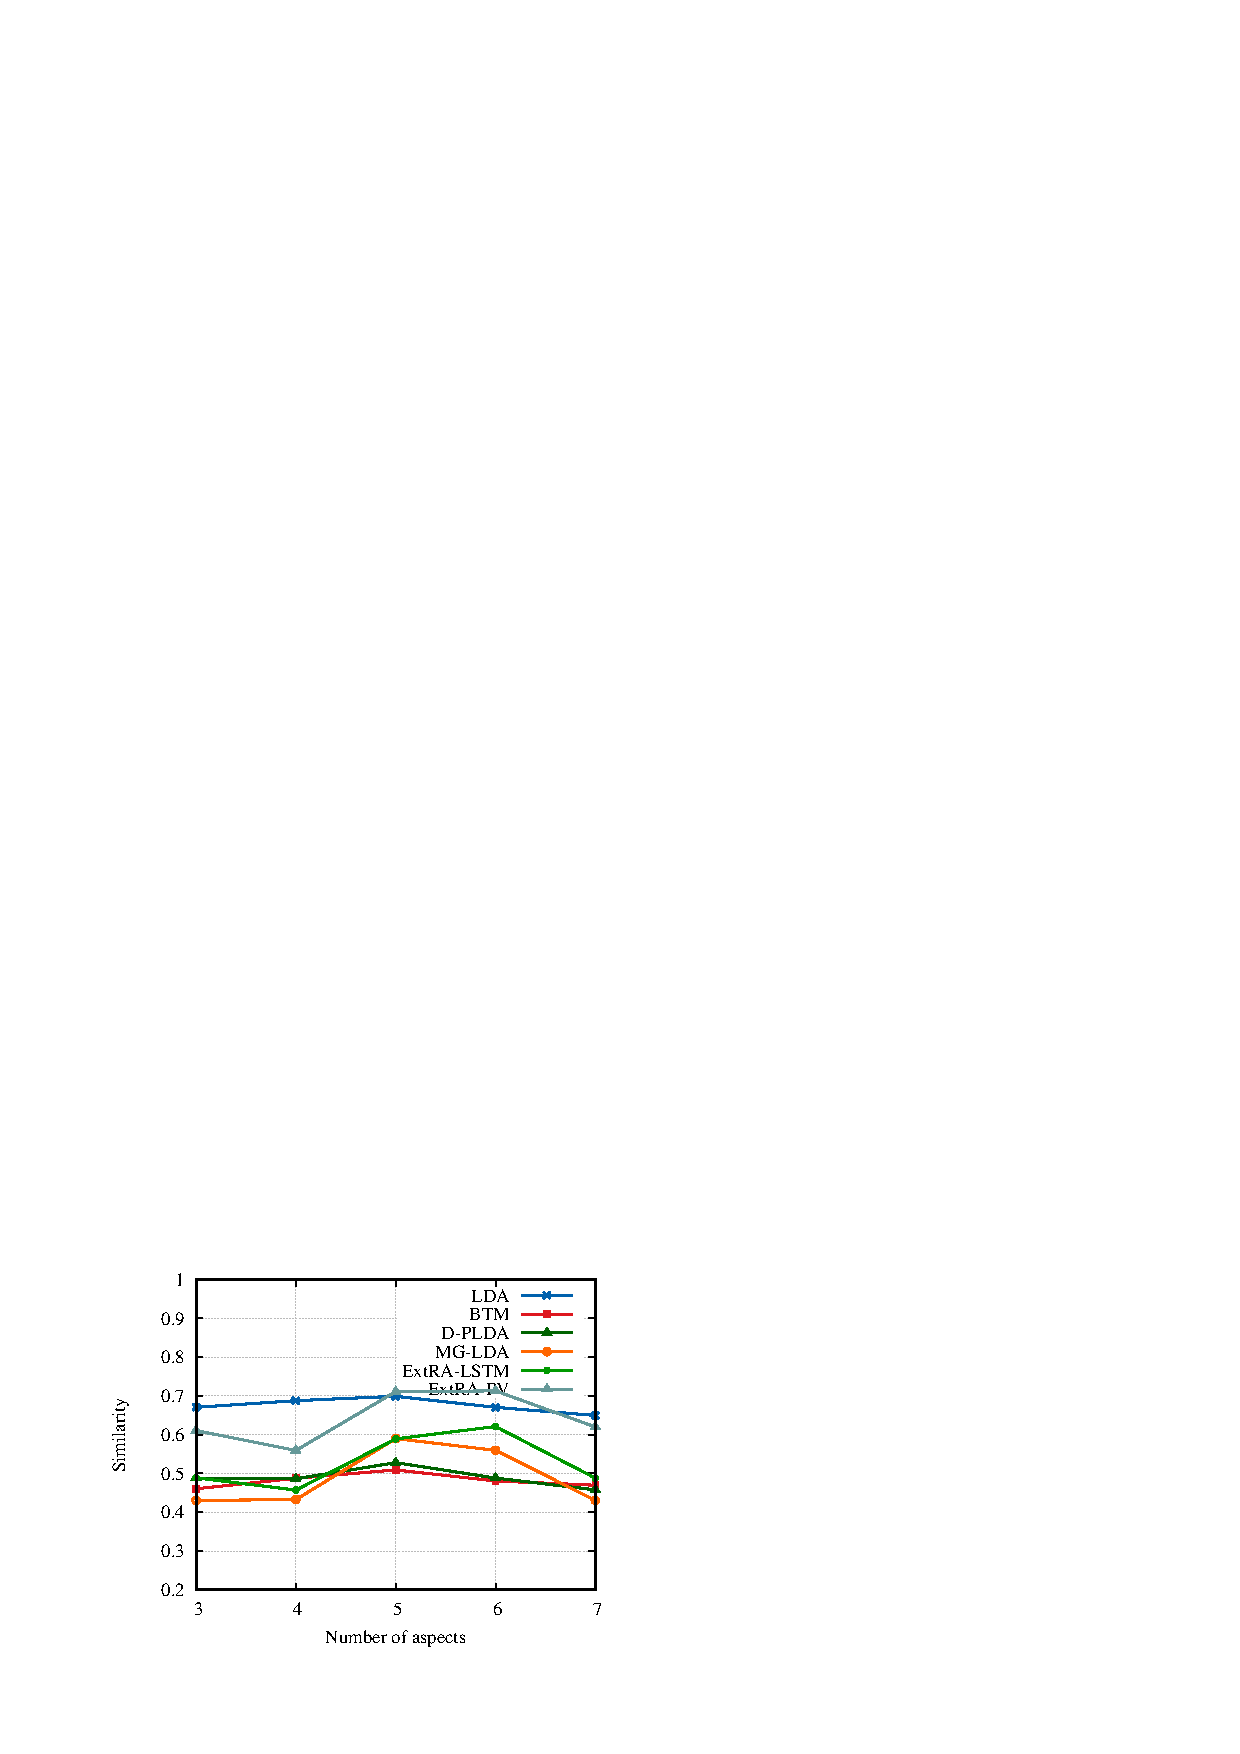
\includegraphics[width=0.8\columnwidth]{data/aspects_hotel}
\hspace*{1cm}
		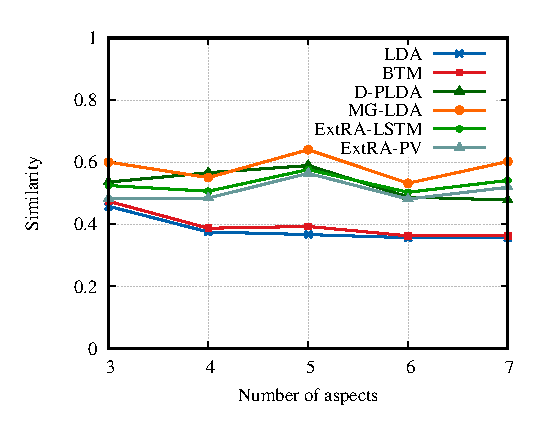
\includegraphics[width=0.8\columnwidth]{data/aspects_mobile}}
	\caption{The performance of different models when adjusting the number of 
		expected aspects $K$. Left: hotel reviews. Right: mobile phone reviews.
		\label{fig:differentk}}
\end{figure*}
\subsubsection{Effect of the Number of Target Prominent Aspects ($K$)}
$K$ reflects the different level of granularity of expected aspects.
A larger $K$ requires the framework to extract 
more fine-grained prominent aspects.
We conduct the experiments using our framework 
with different $K$ ranging from 3 to 7.
From the performance shown in  \figref{fig:differentk},
we can conclude that our framework always outperforms 
other competitors given different $K$ substantially.
\ZY{Fig. 7 change mobile phone to cameras}
%To evaluate the effect of different number of expected aspects, i.e. $K$, which 
%determines the coverage covered by expected aspects,
%we ask our annotators to provide different number of labels on two categories. 
%$K$ ranges from three to seven. 
%The performance of the four models when changing the number of aspects are shown in \figref{fig:differentk}. 
%It can be seen that our models can well extract aspects with variant coverage and perform constantly better than all other models regardless of the number of expected aspects. 


\subsubsection{Effectiveness of the Word Ranking Algorithm}

In the previous experiments, we always use the first approach (word ranking based) to extract the target aspect terms from the ranked topic clusters, other than the experiment with aspect phrases. 
We compare three different ranking setups in this experiment
to show the effectiveness of our proposed ranking method.
%Here we test the effectiveness of several techniques proposed for 
%the ranking step.
%In particular, we compare three setups:
\begin{itemize}
    \item Without word ranking. 
    	 After removing $C-K$ redundant topic clusters, 
    	 we simply select the most important word $w$ associating with highest $m(T,w)$ (mentioned in ~\secref{sec:topicCluster}) 
    	 from each topic cluster $T$.
%          Use directly the word with highest score from aspect cluster after aspect inference.
%          Remove redundant clusters with cluster ranking.
    \item Word ranking without the word importance degrading mechanism.
%    to 
    	We assign the word $w$ within each topic cluster $T_i$ with a score $\text{score}(w,T_i)$ defined in~\eqnref{eq:wordscore}.
    	However, we do not  decrease the importance of terms over iterations (described in \secref{sec:word_ranking}),
    	which prevents our framework from extracting repetitive aspect words
    	  from different topic clusters.
%          As mentioned in \secref{sec:word_ranking}, we do duplicate prevention
%          by considering other clusters when ranking words within a cluster.
%          In this setup we do not include this effort.
    \item Word ranking with the word importance degrading mechanism.
    We rank words within
    each topic cluster and decrease the importance of the words that have been scored before as described in~\eqnref{eq:wordscore}.
\end{itemize}


\begin{table}[t]
	\centering
	\caption{The accuracy performance with different ranking setups.\FX{Needs to be updated to new metrics.}}
	\label{table:rankingeffect}
	\begin{tabular}{|c|C{1.5cm}|C{1.5cm}|C{1.5cm}|}
		\hline
		\diagbox{Type}{Setup} & No word ranking & Word ranking w/o. duplicate prevention & Word ranking w. duplicate prevention \\ \hline
		hotel &0.48 &0.60 & \textbf{0.68} \\ \hline
		mobile phone &0.52 &0.64 & \textbf{0.72} \\ \hline
		mp3 player &0.36 & 0.44 & \textbf{0.52} \\ \hline
		laptop & 0.44 &0.52 & \textbf{0.64} \\ \hline
		camera & 0.43 &0.49 & \textbf{0.58} \\ \hline
		restaurant &0.48 &0.56 & \textbf{0.60} \\ \hline	
	\end{tabular}
\end{table}

%\begin{figure*}[th]
%	\centering
%	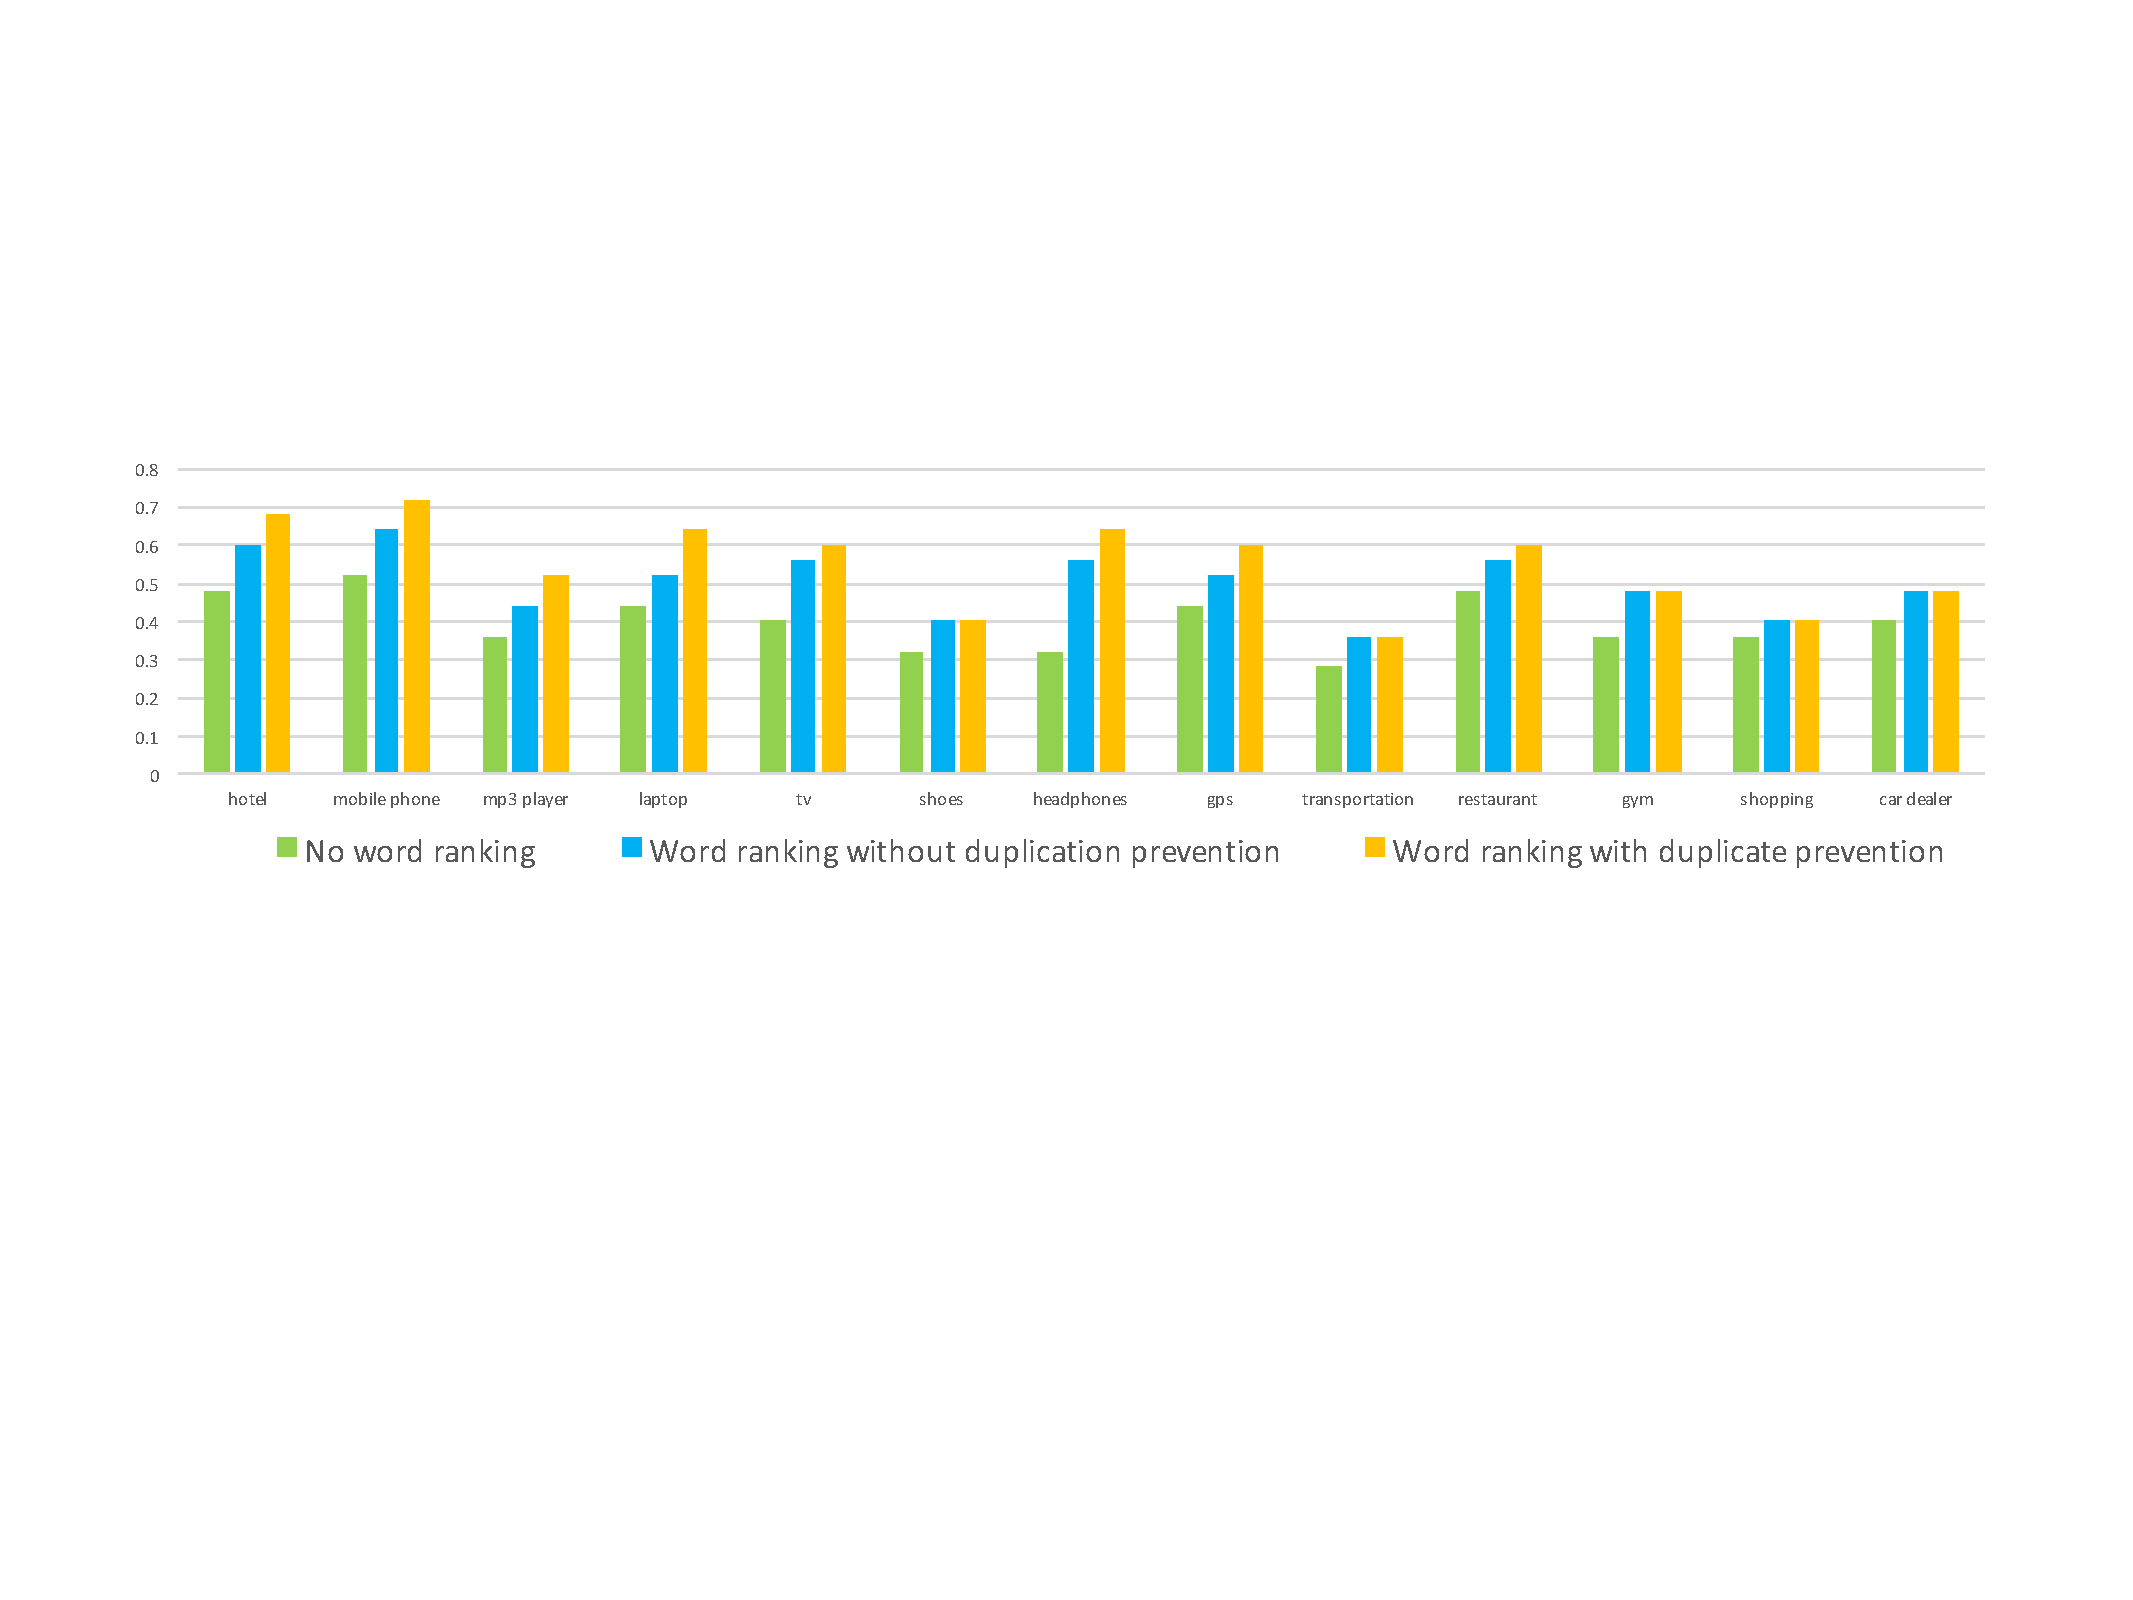
\includegraphics[width=2.0\columnwidth]{figures/rankingeffect}
%	\caption{The accuracy performance with different ranking setups.}
%	\label{fig:rankingeffect}
%\end{figure*}

As shown in \tabref{table:rankingeffect},
we find that: 1) our proposed semantic similarity score for ranking words is indeed effective; 2) the word importance decreasing mechanism improves the prominence of the extracted aspect term.
%the final setup which uses word ranking method 
%cooperated with duplicate prevention
%outperforms others with a substantial margin 
%on all categories.
%has clear advantage across all product categories.

